\documentclass{article}

\usepackage{url}
\usepackage{xcolor}
\usepackage{graphicx}

\setlength{\topmargin}{0in}
\setlength{\textheight}{8.75in}
\setlength{\oddsidemargin}{0.25in}
\setlength{\textwidth}{6.0in}

\providecommand{\cmt}[1]{\textsf{\textcolor{red}{[#1]}}}
\providecommand{\OH}[1]{\mbox{\ensuremath{\mathrm{O}({#1})}}}
\providecommand{\LB}[1]{\mbox{\ensuremath{\mathrm{\Omega}(#1)}}}
\providecommand{\BT}[1]{\mbox{\ensuremath{\mathrm{\Theta}(#1)}}}
\providecommand{\FLOOR}[1]{\mbox{$\lfloor #1 \rfloor$}}

%    for equations with comments on each step (argument gives size of comment box)
\newenvironment{prf}[1]
    {\begin{displaymath}\begin{array}{rclp{#1}}\displaystyle}%
    {\end{array}\end{displaymath}}


\author{Matthias Stallmann}
\title{Software for Multiobjective Optimization in Layered Graphs}
\date{\today}

\begin{document}

\maketitle

\begin{abstract}
  \cmt{overview}
\end{abstract}

\section{Introduction}

\section{Exact Solutions}

Here we discuss mixed integer programming formulations that address
three primary objectives and their bottleneck versions. Using these
formulations it is possible to optimize one objective subject to
restrictions on one or more of the others.
Thus it is possible to identify Pareto optima for any combination of objectives.

Section~\ref{sec:sgf2ilp} describes how a layered graph representation, along with instructions about which objectives are to be optimized or constrained, can be converted to an input file for an ILP solver.
Section~\ref{sec:sol2sgf} discusses a method for converting the (annotated) ILP solution back to a representation that reflects the optimum layout. Section~\ref{sec:galant} introduces an animation/visualization tool that can be used to display the layouts. A detailed example is presented in Section~\ref{sec:case_study}.

\subsection{Integer/Quadratic Programs to Explore Pareto Optima} \label{sec:sgf2ilp}

The \texttt{sgf2ilp.py} program converts a layered graph in sgf format to an integer or
quadratic program in CPLEX\cite{CPLEX} LP format. It supports three different objective functions and their bottleneck versions. Additionally, it also supports optimization of one of the six objective functions given constraints on any of subset of them, including the one being optimized.\footnote{Most solvers will converge more quickly if they are given a known upper bound.} This leads potentially to $6 \cdot 2^6$ possibilities. In the remainder of this section we present the relevant ilp formulations, their complexity in terms of number of variables, constraints, and non-zeroes, as well as experimental results from CPLEX runs.

\subsubsection{ILP and Quadratic Programming Formulations}

The three primary objectives are crossing minimization and two measures of edge offset, \emph{stretch} and \emph{verticality}. Each of the three is based on a specific measure for an edge.
\begin{itemize}
    \item
    \emph{Crossing minimization} counts $c(e)$, the number of times edge $e$ crosses other edges in a given layout. The standard objective is to minimize $(\sum_{e\in E} c(e))/2$, the total number of crossings. The bottleneck version minimizes $\max_{e \in E} c(e)$.
    \item
    \emph{Stretch} assumes that nodes on each layer are equidistant and centered on a layer. Suppose the nodes on a layer are permuted using permutation $\pi$. If the layer has $k$ nodes, the x-coordinate $x(v)$ of node $v$ is
    \begin{eqnarray*}
    (\pi(x)-1) / (k-1) & \mbox{ if } k > 1 \\
    \frac{1}{2} & \mbox{ otherwise }        
    \end{eqnarray*}
    The x-coordinates are treated as being in the interval $[0,1]$, so evenly spaced nodes are at coordinates $0,\frac{1}{k-1},\ldots,\frac{k-2}{k-1},1$. Given this arrangement, the stretch $s(vw)$ of edge $vw$ is defined as $|x(v)-x(w)|$. Two definitions of total stretch exist: assuming the layers are unit distance apart\footnote{It may make more sense to assume the distance between layers is $1/(L-1)$ if there are $L$ layers; this will not affect what we are minimizing.}, we can use the 1-norm to get distance $1+s(vw)$ for edge $vw$ or the Euclidian distance to get $\sqrt{1 + s(vw)^2}$. We can minimize overall distance if we minimize $\sum_{vw\in E} s(vw)$ or $\sum_{vw\in E} s(vw)^2$, respectively. In the bottleneck version we simply minimize $\max_{vw\in E} s(vw)$ either way.
    \item
    \emph{Verticality} assumes nodes are positioned at integer coordinates that need not be contiguous on a layer. If $x(v)$ and $x(w)$ are the coordinates of $v$ and $w$ then $d(v,w) = |x(v)-x(w)|$ is the horizontal displacement of edge $vw$ and $d(v,w)^2$ is the \emph{non-verticality} of $vw$.
    Minimization of non-verticality involves solving a quadratic program. However, there is an integer linear program that achieves the same objective, using the observation that $n^2 = \sum_{i=1}^n (2i-1)$. The bottleneck version minimizes $\max_{vw\in E} d(v,w)$.
\end{itemize}

For the linear/quadratic programs that can optimize/constrain various combinations of these objectives, we use the following variables, all $\geq 0$. Most come from the ILP formulations in previous work, cited below.
Additional variables are introduced later to deal with the multitude of objective combinations.

\begin{prf}{0.72\textwidth}
    x_{i,j} &= & 1 & if node $i$ precedes node $j$ on its layer, 0 otherwise\\
    c_{h,i,j,k} &= & 1 & if edge $hi$ crosses edge $jk$; 0 otherwise; $h<j$ and $i<k$ to avoid double counting \\
    p_{i,\ell} &= & \mbox{integer} & the position, i.e., integer coordinate, of node $i$ on layer $\ell$\\
    d_{u,v,i} &=& \mbox{integer} & used to linearize $d(uv)^2$ \\
    q_{u,v} &=& d(uv)^2 \\
    s_{u,v} &=& s(uv) & (floating point) the stretch $s(uv)$ of edge $uv$ \\
    e_{u,v} &=& 0 & dummy variable to recover edges for an
    \texttt{sgf} representation of the solution
\end{prf}

The constraints can be divided into three categories. First the ones related to crossing minimization.
J\"{u}nger and Mutzel~\cite{1997-JGAA-Juenger} introduced the two-layer versions of these, easily expanded to multiple layers. The addition of constraints for bottleneck crossings is straightforward.
\begin{eqnarray}
    x_{i,j} + x_{j,i} &=& 1 \mbox{ only one node can precede the other} \label{eq:precedes}
    \\
    x_{i,k} - x_{i,j} - x_{j,k} &\geq& -1 \mbox{ for transitivity; $x_{i,j} = x_{j,k} = 1$ implies $x_{i,k}=1$} \label{eq:transitivity}
    \\
    c_{h,i,j,k} - x_{j,h} - x_{i,k} &\geq& -1 \mbox{ condition when edges $hi$ and $jk$ cross } \label{eq:crossing}
    \\
    C - \sum_{h,i,j,k} c_{h,i,j,k} &\geq& 0 \mbox{ to optimize total crossings or constrain them} \label{eq:crossings}
    \\
    C_{bn} - \sum_{h,i} c_{h,i,j,k}- \sum_{h,i} c_{j,k,h,i} &\geq& 0 \mbox{ for all $jk\in E$; bottleneck crossings} \label{eq:bottleneck_crossings}
\end{eqnarray}
To minimize total or bottleneck crossings, simply minimize $C$ or $C_{bn}$, respectively. To put upper bound $\tilde{c}$ on total crossings, add constraint $C \leq \tilde{c}$. Upper bounds on any set of objectives can be added similarly.

Then the ones related to non-verticality, based on Chimani and Hungerla\"{a}nder~\cite{2013-IJC-Chimani}. Here $W$ is the maximum width, number of nodes, on the widest layer.
\begin{eqnarray}
    p_{i,\ell} &\leq& W - 1 \mbox{ positions start at 0, cannot be greater than $W-1$} \label{eq:width}
    \\
    p_{i,\ell} - p_{j,\ell} + W + x_{i,j} &\geq& 1 \mbox{ ensure $p_{i,j}$'s are consistent with $x_{i,j}$'s}\label{eq:consistent}
    \\
    d_{u,v} - p_{u,\ell} - p_{v,\ell+1} &=& 0 \mbox{ linear distance between $u$ and $v$} \label{eq:distance}
    \\
    d_{u,v,i} - d_{u,v} &\leq& i \mbox{ for $1\leq i < W$; setup for linearization} \label{eq:linearization}
    \\
    q_{u,v} - d_{u,v} - \sum_{i=1}^{W-1} 2 d_{u,v,i} &=& 0 \mbox{ uses fact about sum of odd integers} \label{eq:quadratic}
    \\
    NV - \sum_{uv\in E} q_{u,v} &=& 0 \mbox{ total non-verticality} \label{eq:non-verticality}
    \\
    NV_{bn} - q_{u,v} &\geq& 0 \mbox{ for all $uv\in E$; bottleneck non-verticality} \label{eq:bottleneck_nv}
\end{eqnarray}
For non-verticality it is also useful to add lower bounds. If a node $u$ has $k$ neighbors on the layer above (or below) it, the non-verticalities of the corresponding edges must range from 1 to $\FLOOR{k/2}^2$ on one side and 1 to $\FLOOR{(k-1)/2}^2$ on the other. This leads to
\begin{eqnarray}
\sum_{v} q_{u,v} &\geq& \sum_{i=1}^{\FLOOR{(k-1)/2}} i^2 + \sum_{i=1}^{\FLOOR{k/2}} i^2 \label{eq:vlb_one}
\mbox{ ~~~~~ for any $u$ that has outdegree $k$}
\\
\sum_{u} q_{u,v} &\geq& \sum_{i=1}^{\FLOOR{(k-1)/2}} i^2 + \sum_{i=1}^{\FLOOR{k/2}} i^2 \label{eq:vlb_two}
\mbox{ ~~~~~ for any $v$ that has indegree $k$}
\\
NV_{bn} &\geq& \FLOOR{k/2} \mbox{ where $k$ is the maximum indegree or outdegree of any node} \label{eq:bnvlb}
\end{eqnarray}
The lower bounds (\ref{eq:vlb_one}) and (\ref{eq:vlb_two}) are effective even if $NV_{bn}$ is the only relevant objective, but in most cases only if $k > 3$.

Finally the ones related to stretch -- see the 2016 technical report~\cite{2016-TR_Stretch-Stallmann}. These also include (\ref{eq:width}) and (\ref{eq:consistent}), but, instead of the maximum width $W$, we need to consider the width of each separate layer. The current implementation does not allow for combinations of objectives that involve both non-verticality and stretch.
We introduce $z_{i,j}$ for any pair $i,j$ of nodes on adjacent layers and let the constant $W[i]$ represent the width of the layer containing node $i$.
\begin{eqnarray}
  z_{u,v} + \frac{1}{W[i]} p_i - \frac{1}{W[j]} p_j &=& 0 \mbox{ actual difference in centered positions of $i$ and $j$} \label{eq:diff}
  \\
  s_{u,v} + z_{u,v} &\geq& 0 \mbox{ ensure $s_{u,v} \geq |z_{u,v}|$ if $z_{u,v}$ is negative} \label{eq:pos_diff} 
  \\  
  s_{u,v} - z_{u,v} &\geq& 0 \mbox{ ensure $s_{u,v} \geq |z_{u,v|}$ if $z_{u,v}$ is positive} \label{eq:neg_diff}
  \\
  S_{bn} - s_{u,v} &\geq& 0 \mbox{ where $S_{bn}$ is bottleneck stretch}
  \\
  S - \sum_{u,v} s_{u,v} &\geq& 0 \mbox{ if a bound $S$ on total stretch is specified} \label{eq:total_stretch}
\end{eqnarray}

To obtain a desired combination of an objective with a set (possibly empty) of bounds on objectives, \texttt{sgf2ilp.py} has options described in Fig.~\ref{fig:options}.

\begin{figure}
\small
\begin{verbatim}
--objective {total,bottleneck,vertical,bn_vertical,quad_vertical,
             stretch,bn_stretch,quad_stretch}
      minimize ...
        total/bottleneck (total/bottleneck crossings)
        vertical/bn_vertical (minimize total/bottleneck non-verticality)
        quad_vertical (use quadratic programming to minimize non-verticality)
        stretch/bn_stretch (total/bottleneck edge length with evenly spaced nodes)
        quad_stretch (use quadratic programming to miminize total stretch
                      with the stretch of each edge squared)
--total TOTAL
         constraint on the total number of crossings (default: None)
--bottleneck BOTTLENECK
         constraint on the maximum number of crossings of any edge (default: None)
--stretch STRETCH
         constraint on the total edge length (default: None)
--bn_stretch BN_STRETCH
         constraint on the maximum length of any edge (default: None)
--vertical VERTICAL
         constraint on the total non-verticality (default: None)
--bn_vertical BN_VERTICAL
         constraint on the maximum non-verticality of any edge (default: None)
\end{verbatim}

\caption{Options for the \texttt{sgf2ilp.py} program.}
\label{fig:options}
\end{figure}

Only those variables and constraints that are required for the desired objectives are included. However, the $p_{i,\ell}$ and $e_{u,v}$ variables must be included so that an sgf file for the solution can be constructed.

\subsubsection{Sizes of the Integer/Quadratic Programs}

\newcommand{\maxN}{\ensuremath{n_{\max}}}
\newcommand{\maxM}{\ensuremath{m_{\max}}}

In the discussion that follows we introduce relevant notation. Let $n_{\ell}$ be the number of nodes on layer $\ell$ and \maxN\ be the maximum number of nodes on any layer. The \emph{channel} $\ell$, below layer $\ell$, is the set of edges between nodes on layer~$\ell$ and nodes on layer~$\ell-1$. Define $m_{\ell}$ to be the number of edges in channel $\ell$ and \maxM\ to be the maximum number of edges in any channel.

The number of variables for each objective is bounded as follows.
\begin{itemize}
  \item the position variables $p_{i,\ell}$ and the related $x_{i,j}$ are required for all objectives; there are $n$ of the former and \BT{n_{\ell}^2} of the latter on layer $\ell$. Since $\sum_{\ell} n_{\ell}^2$ is \OH{\maxN^2}, the total is \OH{\maxN^2}; the worst case is when there is one large layer, so effectively \OH{n^2}.
  \item the number of crossing variables $c_{h,i,j,k}$ for channel $\ell$ is \BT{m_{\ell}^2} and the sum of these is \OH{\maxM^2}; the worst case arises when there is one large channel, so effectively \OH{m^2}.
  \item the number of variables related to verticality is dominated by the $d_{u,v,i}$'s, so $m\maxN$; usually, $m \geq n$, so this is the dominant term. 
  \item there are exactly $m$ stretch variables $s_{u,v}$; the number of position variables is \OH{n^2} and $m$ is \OH{n^2} as well.
\end{itemize}
The quadratic programming versions of verticality and stretch have no more variables than the linear ones. In the case of verticality, there are no $d_{u,v,i}$ variables so the total is $m$.
The relevant numbers are summarized in Table~\ref{tab:sizes}(a).

The numbers of constraints for each objective are as follows with a summary in Table~\ref{tab:sizes}(b).
\begin{itemize}
  \item for crossings, the dominant constraints are related to transitivity and edge crossings; in the former, every triple of nodes on each layer is involved, so we have $\sum_{\ell} n_{\ell}^3$ with upper bound \OH{n^3}; in the latter, every pair of edges in each channel is involved, so $\sum_{\ell} m_{\ell}^2$, which is \OH{m^2}.
  \item for verticality, the constraints that set values for the $d_{u,v,i}$'s, constraints (\ref{eq:linearization}) dominate, so we have \OH{mn}; if quadratic programming is used, only (\ref{eq:width}), (\ref{eq:consistent}), and (\ref{eq:distance}) are needed, so we have exactly $n$ for (\ref{eq:width}), $\sum_{\ell} n_{\ell}^2$ for (\ref{eq:consistent}), and $m$ for (\ref{eq:distance}); this is \OH{n^2}.
  \item for stretch, sets~(\ref{eq:diff}), (\ref{eq:pos_diff}), and (\ref{eq:neg_diff}) each have one constraint per edge, so the total is \OH{m}; but we also have to have position constraints (\ref{eq:width}) and (\ref{eq:consistent}), so the total is \OH{n^2} based on (\ref{eq:consistent}); only the objective function differs in the quadratic version.
\end{itemize}

The input file size is determined by the total size of all the contraints, i.e., the number of nonzeros in the constraint matrix. These are detailed below with a summary in Table~\ref{tab:sizes}(c).
\begin{itemize}
  \item crossings: constraints (\ref{eq:precedes}), (\ref{eq:transitivity}), and (\ref{eq:crossing}) are constant size and there are \OH{m^2+n^3} of them; constraints (\ref{eq:crossings}) and (\ref{eq:bottleneck_crossings}) are size \OH{m^2} each and there are two of them, so the total is \OH{m^2+n^3}.
  \item verticality: only two constraints have non-constant size; they are the odd integer summations in (\ref{eq:quadratic}) and the total non-verticality constraint (\ref{eq:non-verticality}); of these the summations clearly dominate; there are $m$ constraints, each of size up to $n$, so \OH{mn}; these constraints are not needed for quadratic programming, but the number of position consistency constraints (\ref{eq:consistent}) dominates.
  \item stretch: the only constraint of non-constant size is (\ref{eq:total_stretch}) and it has size $m+1$; again, the position constraints dominate.
\end{itemize}
So the number of nonzeros, while being larger than the number of constraints, is asymptotically the same. The only ones of non-constant size have size equal to the number of some of the constant size constraints.

\begin{table}
  \centering

  \begin{tabular}{c}

\begin{tabular}{|c|c|c|}
  \hline
  objective & detailed & upper bound \\
  \hline
  crossings & $\sum_{\ell} m_{\ell}^2$ & \OH{m^2} \\
  \hline
  verticality & $m\maxN$ & \OH{mn} \\
  \hline
  quadr. verticality & $m$ & \OH{m} \\
  \hline
  stretch/position & $\sum_{\ell} n_{\ell}^2$ & \OH{n^2} \\
  \hline
\end{tabular}
\\ \\
(a) number of variables
\\ \\
\begin{tabular}{|c|c|c|}
\hline
objective & upper bound & dominant constrs.\\
\hline
crossings & \OH{m^2+n^3} & (\ref{eq:transitivity}) and (\ref{eq:crossing}) \\
\hline
verticality & \OH{mn} &  (\ref{eq:linearization})\\
\hline
quadr. verticality & \OH{n^2} & (\ref{eq:consistent})\\
\hline
stretch/position & \OH{n^2} & (\ref{eq:consistent})\\
\hline
\end{tabular}
\\ \\
(b) number of constraints
\\ \\
  \begin{tabular}{|c|c|c|}
    \hline
  objective & upper bound & dominant constraints \\
  \hline
  crossings & \OH{m^2+n^3} & (\ref{eq:transitivity}), (\ref{eq:crossing}) (\ref{eq:crossings}), (\ref{eq:bottleneck_crossings})\\
  \hline
  verticality & \OH{mn} &  (\ref{eq:linearization}) and (\ref{eq:quadratic}) \\
  \hline
  quadr. verticality & \OH{n^2} & (\ref{eq:consistent})\\
  \hline
  stretch/position & \OH{n^2} & (\ref{eq:consistent}) \\
  \hline
\end{tabular}
\\ \\
(c) number of non-zeros
\end{tabular}

\caption{Sizes of integer/quadratic programs.}
\label{tab:sizes}
\end{table}

\subsubsection{Experimental Results}

Experiments were done using CPLEX~version~12.6 on an Intel(R) Xeon(R) Platinum (multi-)processor running Centos~7 Linux.
There are~32 2.1~GHz processors, each with 22~KB cache, and a total of 128~GB shared memory. CPLEX takes full advantage of multiprocessing. In addition to the runtime reported by \texttt{cplex\_ilp}, CPLEX reports the total time taken on all processors, which sometimes an order of magnitude greater. 

\cmt{scatterplots showing nodes/layers and nodes/max edges per channel for north, rome, other, random}

\cmt{include experimental results -- runtimes for each objective as a function of number of edges or max edges in channel.}

\cmt{scatterplots with one of the measures on the x-axis and the other on the y-axis; one series for each objective}

\cmt{report number of nonzeros in relation to max nodes per layer and max edges per channel}

\cmt{report runtimes as a function of number of nonzeros and number of edges per channel; see which measures give more interesting scatterplots}

\subsection{From Solutions to Layouts} \label{sec:sol2sgf}

The next step is to run \texttt{cplex\_ilp} on files generated by \texttt{sgf2ilp.py}. The incantation
\begin{verbatim}
  cplex_ilp -solution -time=LIMIT FILE.lp > FILE.out
\end{verbatim}
will create output with a variety of statistics from the CPLEX run and, more importantly, the values of all variables in the optimum solution found, or best feasible in case of a timeout.
The script \texttt{sol2sgf.py}, a filter from standard input to standard output, can be used to generate an sgf file with the node positions corresponding to the optimum solution. Presence of the dummy $e_{u,v}$ variables means that the original sgf file need not be a separate input. The sgf file produced by \texttt{sol2sgf.py} includes important information such as runtime and the value of the objective function as comments.

\begin{figure}
  \centering

\begin{tabular}{ccc}
  \begin{minipage}{0.35\textwidth}
    \small
  \begin{verbatim}
c a cycle with 6 nodes,
c and 2 layers
t c6 6 6 2
n 0 0 0
n 1 0 1
n 2 0 2
n 3 1 0
n 4 1 1
n 5 1 2
e 0 3
e 0 5
e 1 3
e 1 4
e 2 4
e 2 5
\end{verbatim}
  \end{minipage}
&
  \begin{minipage}{0.25\textwidth}
    \small
  \begin{verbatim}
00-Instance	c6-total
...
runtime 0.027115
...
BeginSolution
total	2
...
p_0_0	0
p_1_0	2
p_2_0	1
p_3_1	1
p_4_1	2
p_5_1	0
e_0_3	0
e_0_5	0
e_1_3	0
e_1_4	0
e_2_4	0
e_2_5	0
...
EndSolution  
\end{verbatim}
\end{minipage}
   &
  \begin{minipage}{0.4\textwidth}
    \small
    \begin{verbatim}
c created 2023/07/06 ...
c from a cplex_ilp solution
c runtime      	0.027115
c TimedOut	0
c SolutionFound	1
c ProvedOptimal	1
c value      	2
t c6-total 6 6 2
n 0 0 0
n 1 0 2
n 2 0 1
n 3 1 1
n 4 1 2
n 5 1 0
e 0 3
e 0 5
e 1 3
e 1 4
e 2 4
e 2 5
\end{verbatim}
\end{minipage}
  \\ \\
  (a)~original sgf file
  &
  (b)~\texttt{cplex\_ilp} output
  &
  (c)~\texttt{sol2sgf.py} output
\end{tabular}

    \caption{Stages in creating an sgf file from a \texttt{cples\_ilp} solution.}
    \label{fig:sol2sgf}
\end{figure}

Fig.~\ref{fig:sol2sgf} shows relevant parts of the process. Fig.~\ref{fig:sol2sgf}~(b) shows only the useful parts of the solution. Values of all other variables are listed in the output as well, preceded by various statistics from the run. The ILP generated by \texttt{sgf2ilp.py} is this case had total crossings as the objective, as evidenced by the value of variable \texttt{total}. Fig.~\ref{fig:c6_drawings} shows the drawings based on the original sgf file and the one based on the results of the pipeline. The next section discusses the generation of the drawings.

\begin{figure}
  \centering
  \begin{tabular}{c c}
    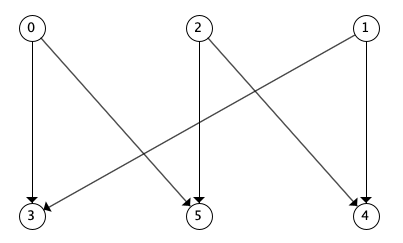
\includegraphics[width=0.49\textwidth]{Images/c6.png}
    &
    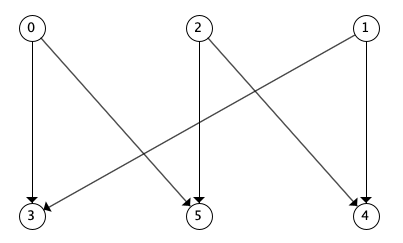
\includegraphics[width=0.49\textwidth]{Images/c6.png}
    \\
    (a)~original positions of \texttt{c6.sfg}
    &
    (b)~after \texttt{cplex\_ilp} and \texttt{sol2sgf.py}
  \end{tabular}
\caption{Drawings of a six-node cycle, before and after crossing minimization.}
\label{fig:c6_drawings}
\end{figure}

\clearpage
\subsection{Visualization using Galant} \label{sec:galant}

Galant~\cite{Galant} is an algorithm animation tool that can also be used to create drawings of graphs, both general graphs and layered. The \texttt{sgf2layeredgraphml.py} script in the \texttt{scripts} directory of the repository creates graphml files designed specifically for display and animation of layered graphs using Galant -- so they may not be useable in other contexts.\footnote{Attributes for nodes include \texttt{layer} and \texttt{positionInLayer} in place of the traditional x- and y-coordinates.} Like the scripts described earlier it reads from standard input and writes to standard output. The Galant repository also includes layered graph algorithms.

\begin{figure}[p]
  \centering
  \begin{tabular}{c@{~~}c}
    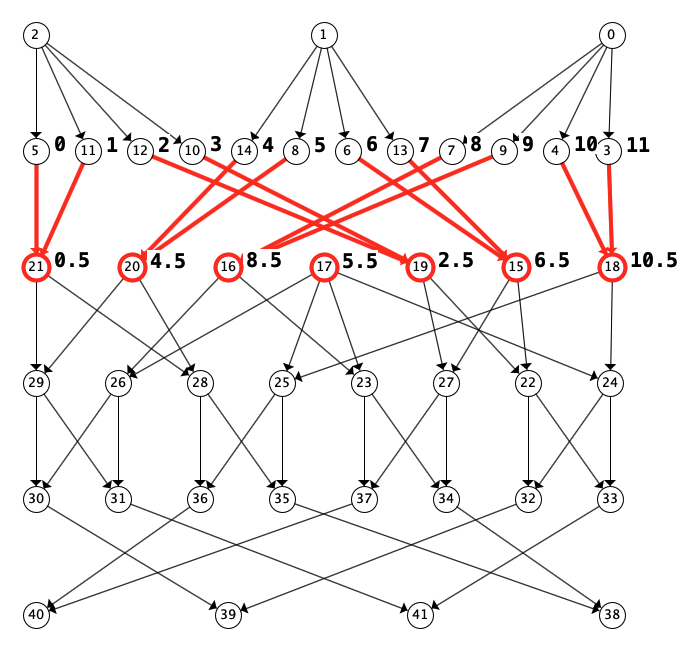
\includegraphics[width=0.49\textwidth]{Images/bary_1}
    &
    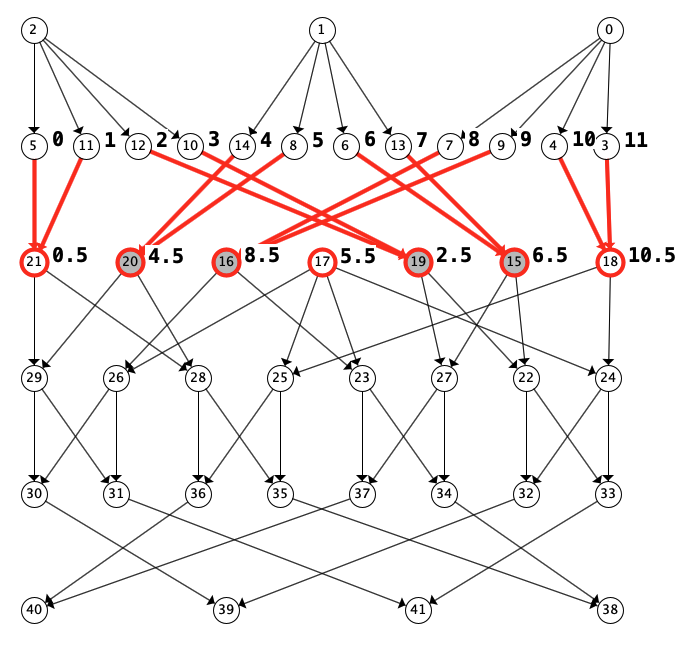
\includegraphics[width=0.49\textwidth]{Images/bary_2}
    \\ \\
    (a)~assigning weights to nodes on a layer
    &
    (b)~marking nodes that will change positions
    \\ \\
    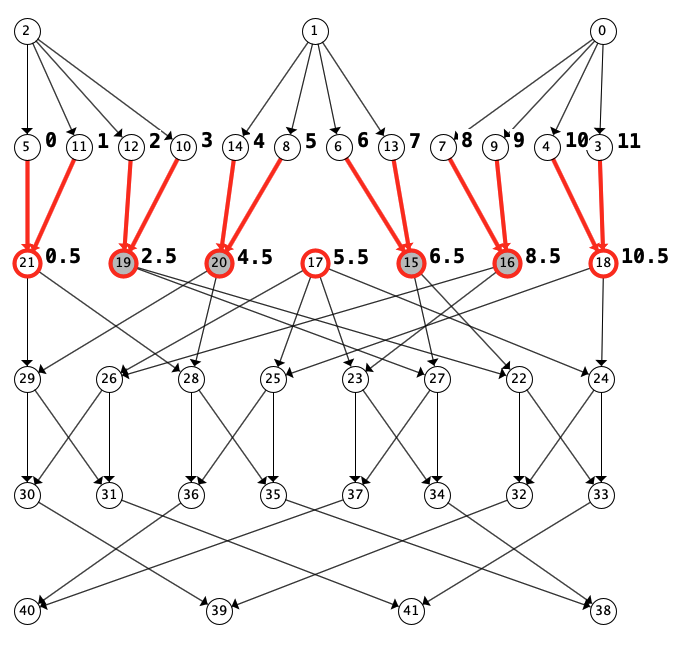
\includegraphics[width=0.49\textwidth]{Images/bary_3}
    &
    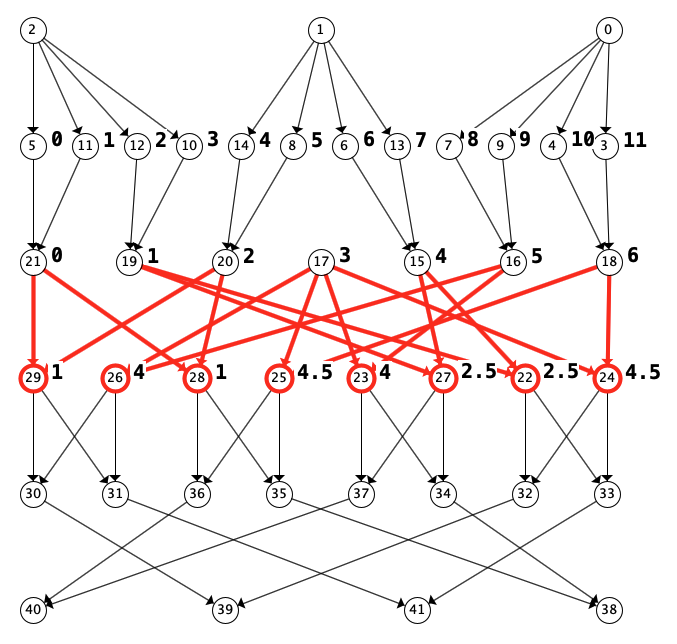
\includegraphics[width=0.49\textwidth]{Images/bary_4}
    \\ \\
    (c)~after sorting by weight 
    &
    (d)~assigning weights on next, lower, layer
  \end{tabular}
  \caption{The Galant animation of the barycenter algorithm in action.}
  \label{fig:barycenter}
\end{figure}

Fig.~\ref{fig:barycenter} illustrates a Galant animation of the barycenter algorithm. A user can step forward or backward in the sequence of displayed steps using the right and left arrow keys, respectively. Holding down the keys will create a movie-like effect. A banner at the top of the window, not shown, displays the current and minimum number of total and bottleneck crossings. Galant animations of barycenter, modified barycenter\footnote{Each pass (i)~identifies the layer~$\ell$ whose incident edges have the most crossings; (ii)~sorts $\ell$ based on positions of neighbors on layers both above and below; (iii)~does an upward sweep starting with layer $\ell+1$ and a downward one starting with $\ell-1$.}, sifting~\cite{1999-GD-Matuszewski-p217}, and mce~\cite{2012-JEA-Stallmann} are in the Research/Layered-Graphs/Algorithms directory of the repository. The parallel Graphs directory has example graphs.
The animations are easy to develop; they are essentially Java programs with a straightforward API that accesses both standard layered graph operations, such as assigning weights and sorting, along with simple animation effects.

\subsection{A Case Study in Seven Drawings} \label{sec:case_study}

Here we illustrate how our software is used to create eight different drawings of the same graph, \texttt{North42.32}, one of over a thousand graphs collected by Stephen North, as layered using an algorithm of Gansner et al.\cite{1993-IEEE_SE-Gasner}. The first set of four illustrates tradeoffs between total and bottleneck crossings; the second set show tradeoffs between crossings and verticality.
In both cases the script \texttt{sgf2opt.sh} identifies the extreme points of the Pareto frontier and \texttt{pareto\_frontier.sh} finds the remaining points.

\subsubsection{Total Crossings versus Bottleneck Crossings}

First a run of \texttt{sgf2opt.sh}.\footnote{It is best to run the scripts within a directory containing the sgf input, being aware that multiple files will be created in the process. Each script invocation needs to be preceded by the path to \emph{repository}/\texttt{ilp}.} The \texttt{North42.32} instance is in file \texttt{north42.32.sgf}.
\begin{verbatim}
    sgf2opt.sh north42.32.sgf total bottleneck 7200
\end{verbatim}
The last numerical argument is optional; it specifies a time limit for the CPLEX runs in seconds -- default is one hour: here we allow two hours. In the descriptions below, assume that \texttt{cplex\_ilp} has an additional flag \texttt{-time=7200}. The script creates four integer programs and solves them using \texttt{cplex\_ilp}, a frontend for CPLEX.\footnote{Available at \texttt{https://github.com/mfms-ncsu/CPX-ILP}.}
The first two runs establish the minimum number of total and bottleneck crossings, respectively, using the \texttt{sgf2ilp.py} script to generate the ILP's, and creating output files from the CPLEX runs.
{\small
\begin{verbatim}
sgf2ilp.py --objective total < north42.32.sgf > north42.32-total.lp
cplex_ilp -solution north42.32-total.lp > north42.32-total.out
sgf2ilp.py --objective bottleneck < north42.32.sgf > north42.32-bottleneck.lp
cplex_ilp -solution north42.32-bottleneck.lp > north42.32-bottleneck.out
\end{verbatim}
}
The \texttt{-solution} flag tells \texttt{cplex\_ilp} to output values of variables in a format that allows later conversion to an sgf file.
The script harvests the objective values from these two runs: 44~for minimum total crossings and 3~for minimum bottleneck crossings. Then it runs
{\small
\begin{verbatim}
sgf2ilp.py --objective total --bottleneck 3 < north42.32.sgf > north42.32-bottleneck_3_total.lp
cplex_ilp -solution north42.32-bottleneck_3_total.lp > north42.32-bottleneck_3_total.out
sgf2ilp.py --objective bottleneck --total 44 < north42.32.sgf > north42.32-total_44_bottleneck.lp
cplex_ilp -solution north42.32-total_44_bottleneck.lp > north42.32-total_44_bottleneck.out
\end{verbatim}
}
The output summarizes the outcome, showing that, when bottleneck crossings are bounded by~3, total crossings have minimum~46; and when total crossings are bounded by~44, bottleneck crossings have minimum~7. We can then do another run to establish an intermediate Pareto point if one exists.
{\small
\begin{verbatim}
sgf2ilp.py --objective bottleneck --total 45 < north42.32.sgf > north42.32-total_45_bottleneck.lp
cplex_ilp -solution north42.32-total_45_bottleneck.lp > north42.32-total_45_bottleneck.out
\end{verbatim}
}
When total crossings are bounded by~45, bottleneck crossings have minimum~5.

\begin{figure}[p]
    \centering
    \begin{tabular}{c@{~~}c}
      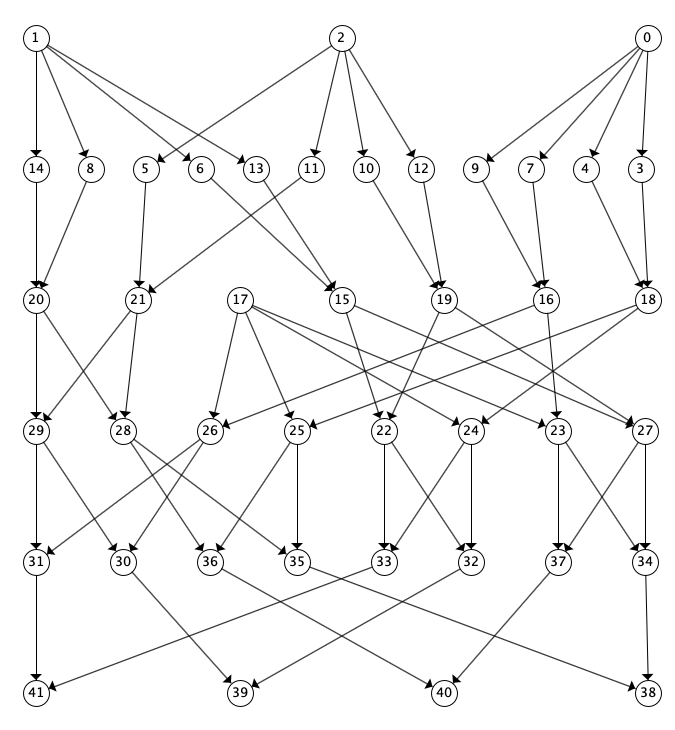
\includegraphics[width=0.49\textwidth]{Images/n42-t44b7}
      &
      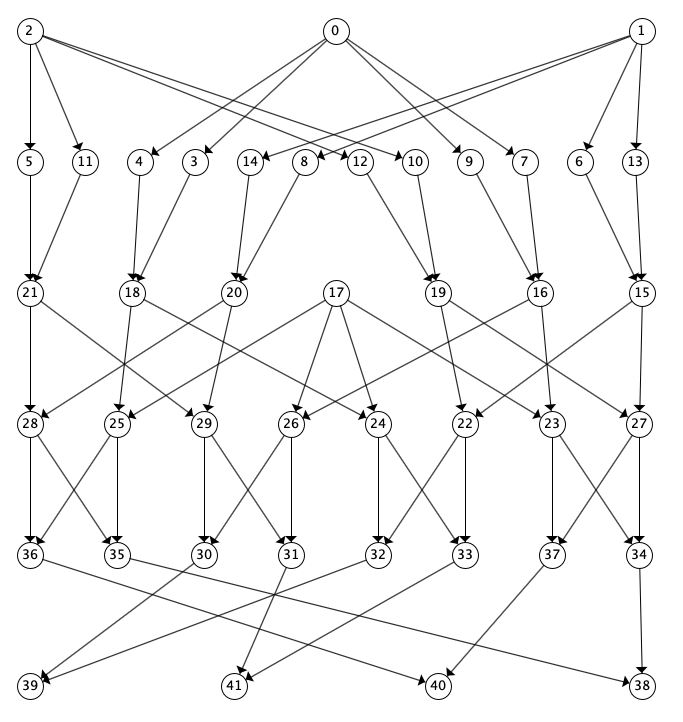
\includegraphics[width=0.49\textwidth]{Images/n42-t45b5}
      \\
      (a) 44~crossings, 7~bottleneck crossings
      &
      (b) 45~crossings, 5~bottleneck crossings
    \end{tabular}

    \bigskip
    \begin{tabular}{c}
      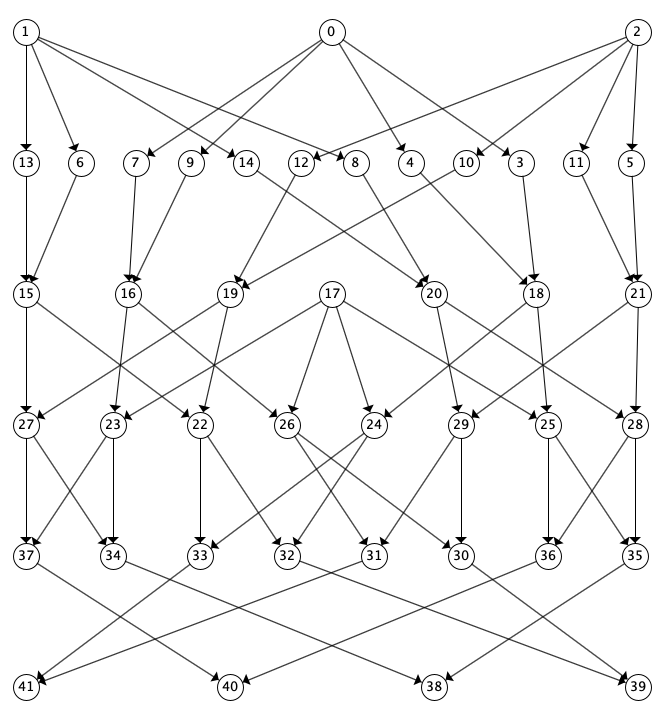
\includegraphics[width=0.49\textwidth]{Images/n42-t46b3}
      \\
      (c) 46~crossings, 3~bottleneck crossings
    \end{tabular}

    \bigskip
    \caption{Three drawings of \texttt{north42.32\_GKNV}, showing all possible tradeoffs between total crossings
    and bottleneck crossings.}
    \label{fig:north42_bt}
  \end{figure}

Fig.~\ref{fig:north42_bt} illustrates these Pareto optima. To generate these pictures, we first do
{\small
\begin{verbatim}
sol2sgf.py < north42.32-total_44_bottleneck.out > north42.32-total_44_bottleneck.sgf
sol2sgf.py < north42.32-total_45_bottleneck.out > north42.32-total_45_bottleneck.sgf
sol2sgf.py < north42.32-bottleneck_3_total.out > north42.32-total_46_bottleneck.sgf
\end{verbatim}
}
to create sgf files from the solutions embedded in the \texttt{cplex\_ilp} output.

Finally, the \texttt{scripts} directory in the repository has \texttt{sgf2layeredgraphml.py}, used to create inputs for Galant.
{\small
\begin{verbatim}
sgf2layeredgraphml.py < north42.32-total_44_bottleneck.sgf > north42.32-total_44_bottleneck.graphml
sgf2layeredgraphml.py < north42.32-total_45_bottleneck.sgf > north42.32-total_45_bottleneck.graphml
sgf2layeredgraphml.py < north42.32-total_46_bottleneck.sgf > north42.32-total_46_bottleneck.graphml
\end{verbatim}
}
Of course, the names can be shortened along the way and the suffixes can include information about both objectives, as in \texttt{t44b7}, \texttt{t45b5}, and \texttt{t46b3}.

\clearpage

\subsubsection{Total Crossings versus Non-Verticality}

To explore tradeoffs between total crossings and non-verticality, we begin with
{\small
\begin{verbatim}
  sgf2opt.sh north42.32.sgf total vertical [runtime]
\end{verbatim}
}
Results give the two extreme points: with minimum total crossings,~44, the minimum achievable non-verticality is~172; with minimum non-verticality, 150, total crossings are minimized at~48. This leaves three potential intermediate Pareto points. We can use the script \texttt{pareto\_frontier.sh} to explore these as follows.
\begin{verbatim}
  pareto_frontier vertical total 45 47 [runtime]
\end{verbatim}
which runs
{\small
\begin{verbatim}
sgf2ilp.py --objective bottleneck --total N < north42.32.sgf > north42.32-total_N_bottleneck.lp
cplex_ilp -solution north42.32-total_N_bottleneck.lp > north42.32-total_N_bottleneck.out
\end{verbatim}
}
for \texttt{N} = 45--47. The results, along with the extreme points, give us the following $(tc,nv)$ pairs, where $tc$ is total crossings and $nv$ is (total) non-verticality: (44,172), (45,158), (46,152), (47,152), and (48,150). The pair (47,152) is not a Pareto optimum; it is dominated by (46,152). The drawings in Fig.~\ref{fig:north42_tv} were generated using the same scripts as those in Fig.~\ref{fig:north42_bt}. An argument can be made that the two intermediate drawings, (b) and (c), are more aesthetically pleasing than the extremes.

\begin{figure}[p]
    \centering
    \begin{tabular}{c@{~~}c}
      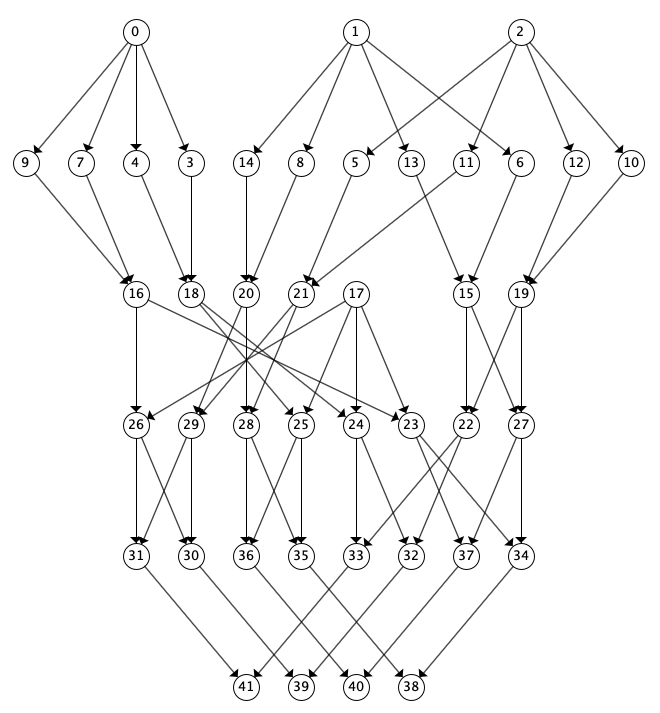
\includegraphics[width=0.49\textwidth]{Images/n42-t44v172}
      &
      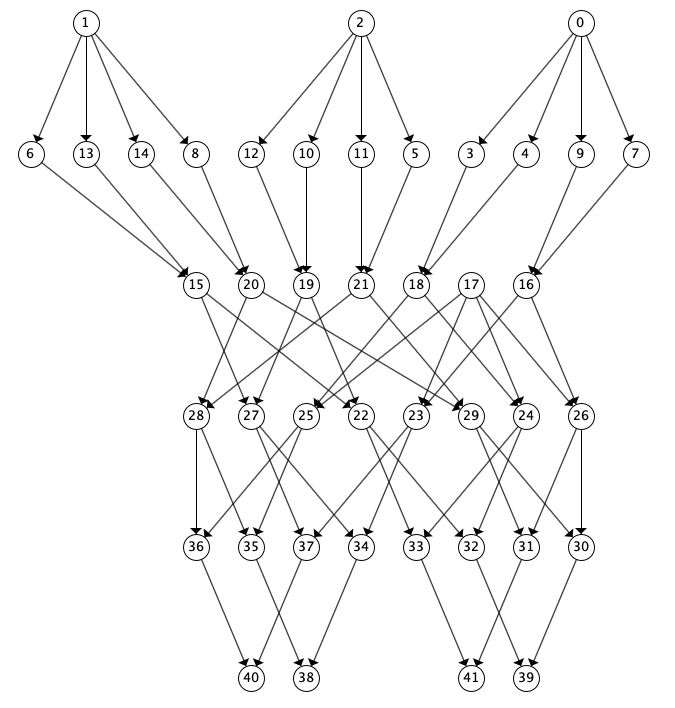
\includegraphics[width=0.49\textwidth]{Images/n42-t45v158}
      \\ \\
      (a) 44~crossings, non-verticality$=172$
      &
      (b) 45~crossings, non-verticality$=158$
      \\ \\
      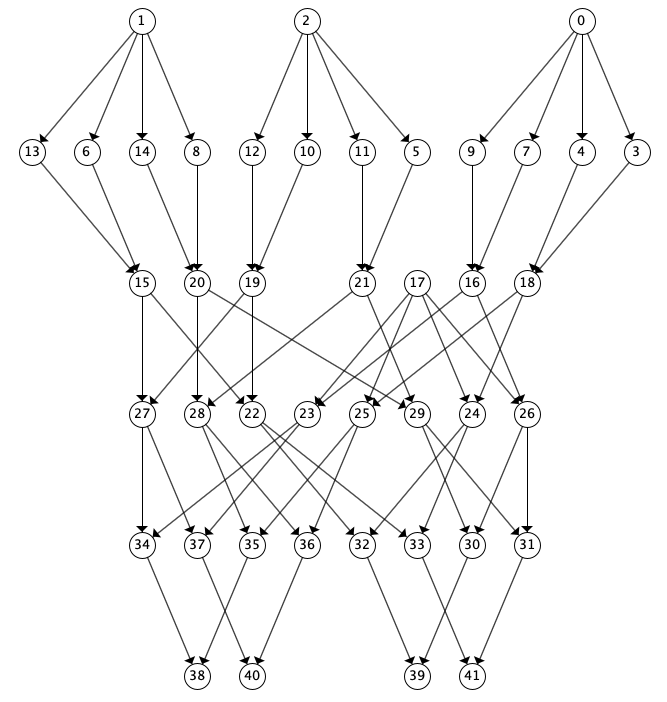
\includegraphics[width=0.49\textwidth]{Images/n42-t46v152}
      &
      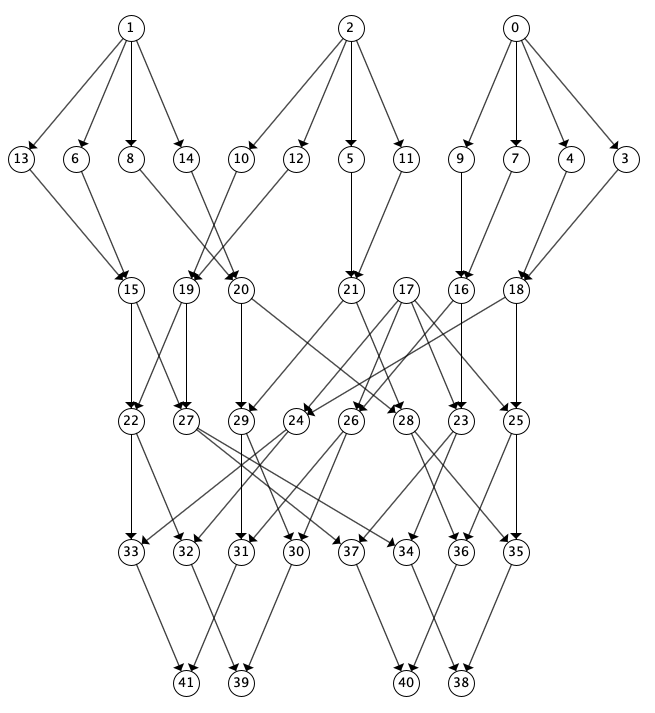
\includegraphics[width=0.49\textwidth]{Images/n42-t48v150}
      \\ \\
      (c) 46~crossings, non-verticality$=152$
      &
      (d) 48~crossings, non-verticality$=150$
    \end{tabular}
    \caption{Four drawings of \texttt{north42.32\_GKNV}, showing all possible tradeoffs between total crossings
    and non-verticality.}
    \label{fig:north42_tv}
\end{figure}

\clearpage


\section{Heuristics}

Here we describe software that implements a large collection of simple
heuristics targeting the various layered graph objectives.

\subsection{Iterative improvement}

Iterative improvement heuristics start with a given configuration, random or the result of preprocessing -- see Section~\ref{sec:preprocessing}, and perform rearrangements until a stopping criterion is achevied.
Each heuristic defines an \emph{iteration}, a single rearrangement of nodes on a layer, and a \emph{pass}, a sequence of iterations that either systematically rearrange every layer or every single node.
Heuristics terminate either after a fixed number of passes or when a pass fails to improve the objective or any of a set of objectives.

\subsubsection{Basic paradigms}

There are two basic types of iterative improvement heuristics: sorting and node-insertion.

\medskip
\noindent \textbf{Sorting.}
Each iteration of a sorting heuristic works as follows.
\begin{enumerate}
        \item choose a layer $k$
        \item assign weights to nodes on layer $k$ based on positions of their neighbors on layers $k-1$ and/or $k+1$
        \item sort the nodes on layer $k$ by increasing weight
\end{enumerate}

Examples of sorting heuristics are the median and the barycenter heuristics -- see~\cite{1999-DiBattista}.
Let $L$ be the number of layers.
Then in both of these heuristics a pass consists of an \emph{upsweep}, where $k=2,\ldots,L$ and weights are based on layer $k-1$, followed by a \emph{downsweep}, where $k=L-1,\ldots,1$ and weights are based on layer $k+1$.
The difference is that the in the median heuristic, the weight of $x$ is the median of the positions of its neighbors, whereas in the barycenter it is the mean.

In a variant called \emph{mod-bary}, the survivor among several variants of \emph{maximum crossings layer}~\cite{2008-MSThesis-Gupta}, each pass works as follows.
\begin{enumerate}
    \item choose unmarked layer $k^*$ whose incident edges have the maximum number of crossings and mark it
    \item sort nodes on layer $k^*$ with weights based on neighbor positions on layers $k^*-1$ (if $k^* >1$) \emph{and} $k^*+1$ (if $k^*<L$)
    \item do an upsweep for layers $k^*+1,\ldots,L-1$
    \item do a downsweep for layers $k^*-1,\ldots,1$
    \item the pass ends when all layers are marked
\end{enumerate}
In many cases mod-bary outperforms barycenter (which, in turn, almost always outperforms the median heuristic).

\medskip
\noindent \textbf{Node-insertion.}
Each pass of a node-insertion heuristic works as follows.
\begin{enumerate}
    \item choose unmarked node $x$
    \item put $x$ into an optimal position on its layer based on some objective, shifting other nodes as needed
\end{enumerate}

The first published node-insertion heuristic, called \emph{sifting}, is due to Matuszewski et al.~\cite{1999-GD-Matuszewski-p217}. In their version no marking takes place.
Nodes are simply considered by increasing or decreasing degree in each pass.
Each $x$ in turn is moved to a position that minimizes total crossings.
The heuristic switches to the opposite order when a pass does not yield improvement.

Another node-insertion heuristic, specifically designed for the bottleneck crossing problem, is \emph{maximum crossings edge (mce)}~\cite{2012-JEA-Stallmann}. To choose node $x$, the mce heuristic first identifies the edge $vw$ with the maximum number of crossings, making sure that at least one of $v,w$ is unmarked. Then $v$ and/or $w$ is moved. Suppose $x=v$ is moved. Instead of moving $x$ to a position that minimizes the total number of crossings overall, as sifting does, mce moves $x$ to a position that minimizes the maximum number of crossings for any edge incident on $x$.

A simpler version of mce, which targets total crossings, is \emph{maximum crossings node (mcn)} (see Gupta~\cite{2008-MSThesis-Gupta}). Here $x$ is the node whose incident edges have the most crossings and, as in sifting, $x$ is moved to the position that minimizes total crossings.

The mce and mcn heuristics motivate two other variations: mce-t, where $x$ is chosen as in mce but the position of $x$ is chosen to minimize total crossings; and mcn-e, where $x$ is the (unmarked) node with the maximum number of crossings but the position of $x$ is based on minimizing the maximum number of crossings for any edge incident on $x$. 

\subsection{Verticality}

Optimizing verticality, i.e., minimizing non-verticality, requires special care.
When $n_{\ell}$, the number of nodes on layer $\ell$ is less than $W$, the largest number of nodes on any layer, the positions of nodes on layer $\ell$ may not be contiguous.
This means that the sorted order of nodes on $\ell$ does not uniquely determine node positions and placing a node in its optimum position on layer $\ell$ may not involve shifting of other nodes.

\subsubsection{Vertical barycenter}

We implemented a non-verticality-minimizing heuristic based on mod-bary, called \emph{vertical-bary}. Each iteration starts the same way as in mod-bary, with $k^*$ the layer whose incident edges have maximum total nonverticality. Then, to choose positions based on the sorted order, we can apply a dynamic programming algorithm that chooses optimum positions for layer $\ell$ given fixed positions on the relevant neighboring layers and the sorted order of nodes on the current layer $\ell$.
The relevant neighboring layers are $\ell-1$ and $\ell+1$ if $\ell=k^*$ and either $\ell-1$ or $\ell+1$ otherwise.

Let $d_{x,p}$ be the nonverticality induced by putting node $x$ in position $p$ on layer $\ell$ and let $p^*(x)$ be the position of $x$ in an assignment of positions that minimizes $\sum_{x ~\mathrm{on}~ \ell} d_{x,p^*(x)}$. Our goal is to find $p*(x)$ for all $x$ on $\ell$.

Let $C[i,j]=$ the minimum total nonverticality for nodes $1,\ldots,i$ (in the sorted order) using positions $1,\ldots,j$ only, and let $P[i,j] =$ \textbf{true} if the optimum position for $i$ is $j$, \textbf{false} otherwise.
Starting with $C[0,0]=0$ and $C[j,0]=\infty$ for all $j$ as base cases, $C[i,j]$ is the minimum of
\begin{eqnarray*}
C[i-1,j-1] + d_{i,j} && \mbox{ put node } i \mbox{ in position } j
\\
C[i,j-1] && \mbox{ put node } i \mbox{ in a position } < j
\end{eqnarray*}
If the first option is minimum, then $P[i,j] =$ \textbf{true}, otherwise $P[i,j] =$ \textbf{false}.

Note that the desired total nonverticality is $C[n_{\ell},W]$ and we only need $i \leq j \leq W$ and $i \leq n_{\ell}$.
The number of table entries in a dynamic programming algorithm, ignoring the base cases, is therefore $n_{\ell} (W - n_{\ell})$, the worst case being when $n_{ell}\approx W/2$.

To extract $p^*(i)$ for $i = 1, \ldots, n_{\ell}$ apply the following recursive procedure starting with Positions($n_{\ell},W$).

\begin{tabbing}
    xxx \= xxx \= xxx \= xxx \= xxx \= xxx \= xxx \= xxx
            \= \kill
\textbf{procedure} Positions($i,j$) \\
\>\textbf{if} $i=0$ \textbf{return} \\
\>\textbf{if} $P[i,j]$ \\
\>\>$p^*(i) =j$ \\
\>\>Positions($i-1,j-1$) \\
\>\textbf{else} \\
\>\>Positions($i,j-1$) \\
\textbf{end}
\end{tabbing}

\subsubsection{Maximum nonverticality edge}

The \emph{maximum nonverticality edge (mnve)} heuristic behaves in a way similar to mce with the following observations.
\begin{itemize}
    \item It is more like mce-n in that it positions node $x$ to minimize total nonverticality.
    \item The optimum position for $x$ could be unoccupied: in that case no shifting takes place.
\end{itemize}
A variant that minimizes the maximum nonverticality among edges incident on $x$ with target objective bottleneck nonverticality could be easily implemented.

\subsection{Combining heuristics}

\subsection{Preprocessing} \label{sec:preprocessing}

Experiments have shown that preprocessing the graph before applying an iterative improvement heuristic leads to better and more consistent results.
The most effective techniques involve depth-first or breadth-first search
followed with a sort of each layer by increasing discovery time of the nodes.
For two-layer instances breadth-first search, particularly a guided two-pass version, is especially effective -- see~\cite{2001-JEA-Stallmann}.
With more layers depth-first search is a better choice.

The sorting based on these graph traversals brings nodes that are close to each other in the graph near each other on their respective layers.

\subsection{Post processing}

\cmt{for large scale experimental results using mod-bary with iterative improvement heuristics, go to the research drive \texttt{rs1} and look under\\
Old-Research/Layered-Graphs-Old/LargeScale-Experiments}


\section{Random Generation}

\section{Conclusions}

\section*{Acknowledgements}

Several students have contributed to this work either as developers and experimenters.
Saurabh Gupta, in research leading to his 2008 master's thesis, implemented the first version of what is now \texttt{minimization}. It incorporated a large variety of heuristics including, among others: barycenter, median, mod-bary, sifting, mcn, and dfs.

In later independent study projects, Venkata Uday K. Sonthy (2014) implemented programs and scripts to convert layered graphs to ILP's for crossing minimization and extracting solutions; Weijia Li (2016) explored tradeoffs between stretch and crossings (including their bottleneck versions), adding necessary heuristics;
Mason Hicks (2022) added implementations of heuristics for minimizing nonverticality. All of these students undertook large scale experiments.

We also acknowledge the computing resources provided by North Carolina State University High Performance Computing Services Core Facility (\texttt{RRID:SCR\_022168}).

\bibliographystyle{plain}

\bibliography{layered_graph_papers}

\end{document}
